%--------------------
% Packages
% -------------------
\documentclass[11pt,a4paper,titlepage]{article}
\usepackage[utf8]{inputenc}
\usepackage[T1]{fontenc}
\usepackage{outlines}
\usepackage{booktabs}
\usepackage{mathptmx} % Use Times Font
\usepackage{subcaption}

\usepackage[pdftex]{graphicx} % Required for including pictures
\usepackage[pdftex,linkcolor=black,pdfborder={0 0 0}]{hyperref} % Format links for pdf
\usepackage{calc} % To reset the counter in the document after title page
\usepackage{enumitem} % Includes lists

\frenchspacing % No double spacing between sentences
\linespread{1.2} % Set linespace
\usepackage[a4paper, lmargin=0.1666\paperwidth, rmargin=0.1666\paperwidth, tmargin=0.1111\paperheight, bmargin=0.1111\paperheight]{geometry} %margins

\usepackage[all]{nowidow} % Tries to remove widows
\usepackage[protrusion=true,expansion=true]{microtype} % Improves typography, load after fontpackage is selected
\usepackage{csquotes}
\usepackage[style=ieee,backend=bibtex]{biblatex}
\addbibresource{bibliography.bib}

%-----------------------
% Set pdf information and add title, fill in the fields
%-----------------------
\hypersetup{ 	
pdfsubject = {COM00032H},
pdftitle = {MLPG Open Assessment},
pdfauthor = {Y3843100}
}

\title{MLPG Open Assessment COM00032H}


\author{Exam No: Y3843100}

\date{\today}
%-----------------------
% Begin document
%-----------------------
\begin{document}


\maketitle


\section{Conditional independence in Bayesian networks}

\paragraph{Independent pairs}
\[I = \{(A,C),(A,E),(A,F),(B,C),(B,E),(B,F),(D,C),(D,E),(D,F)\}\]

\paragraph{Independent pairs conditioned on \(Z = \{C,G\}\)}

\[I = \emptyset\]

\paragraph{Markov equivalent DAG}
Reverse edges but maintain immoralities, i.e. change \(B\) edges \textit{fig \ref{fig:1.3}}

\begin{figure}[htb]
  \centering
    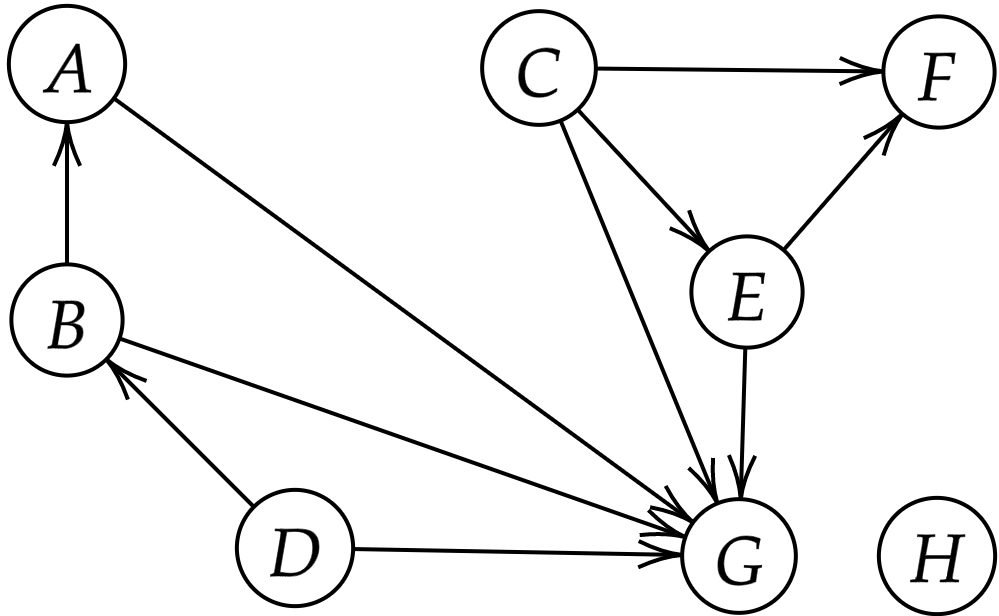
\includegraphics[width=0.5\textwidth]{../q1/fig13.png}
    \caption{Question 1.3 Markov equivalent DAG}
  \label{fig:1.3}
\end{figure}

\paragraph{Non-Markov equivalent DAG}
Change immoralities. I.e. reverse all edges from \(G\) \textit{fig \ref{fig:1.4}}
\begin{figure}[htb]
  \centering
    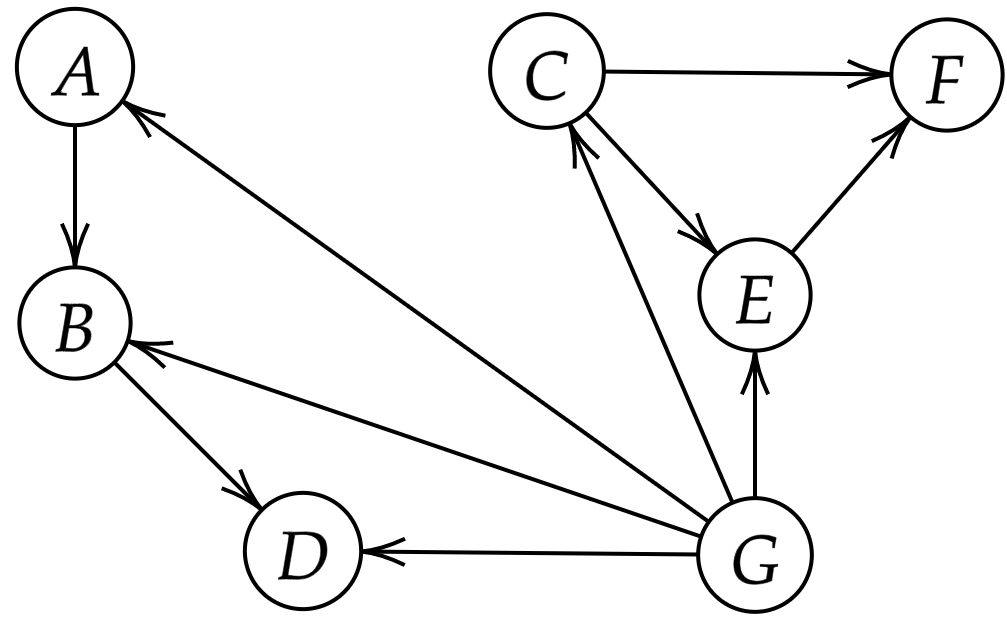
\includegraphics[width=0.5\textwidth]{../q1/fig14.png}
    \caption{Question 1.4 Non-Markov equivalent DAG}
  \label{fig:1.4}
\end{figure}

\section{House prices with STAN}
%TODO: Offload all data manipulation in the .py files and not in the q2data
%TODO: Make sure all files embedded the model as a str
  \subsection{A simple model (figs \ref{fig:2.1} and \ref{tab:2.1})}
  %Say 95 confidence interval compared to the mean is pretty solid. (i.e. the interval is tight around the mean + talk about SD)
%TODO: Say something about "Explain what steps you have taken to ensure that you have computed reasonable approximations to the true posterior distributions over your parameters." in respect to the plots, conf interval, etc
  We can state that our estimated posteriors approximate the true distributions as all chains have converged \(\hat{R} = 1\), which is also observed by the beta plot. The preference for MCMC sampling over variational inference was due to the fact that the size of our dataset and the length of this assessment permits the usage of the more computationally intensive method. In addition, the asymptotic correctness of the posterior justifies the larger computational expense \parencite{BleiVI}. Empirical tests show that the STAN default of 1000 iterations (2000 samples) and 4 chains is enough for convergence.
  %This model asserts the assumption that althought the data represents the house prices of two distinct locations, the price formation given Age and Size is the same for the two regions.

  \begin{figure}[htb]
    \centering
      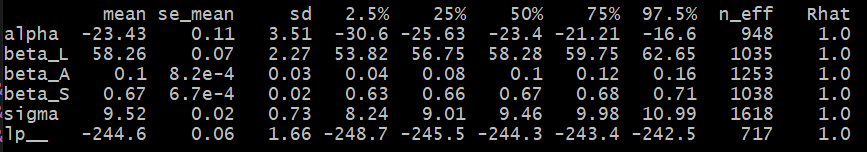
\includegraphics[width=\textwidth]{../q21/q21_summary_table.png}
      \caption{Question 2.1 posterior table summary}
    \label{tab:2.1}
  \end{figure}

  \begin{figure}[htb]
    \centering
      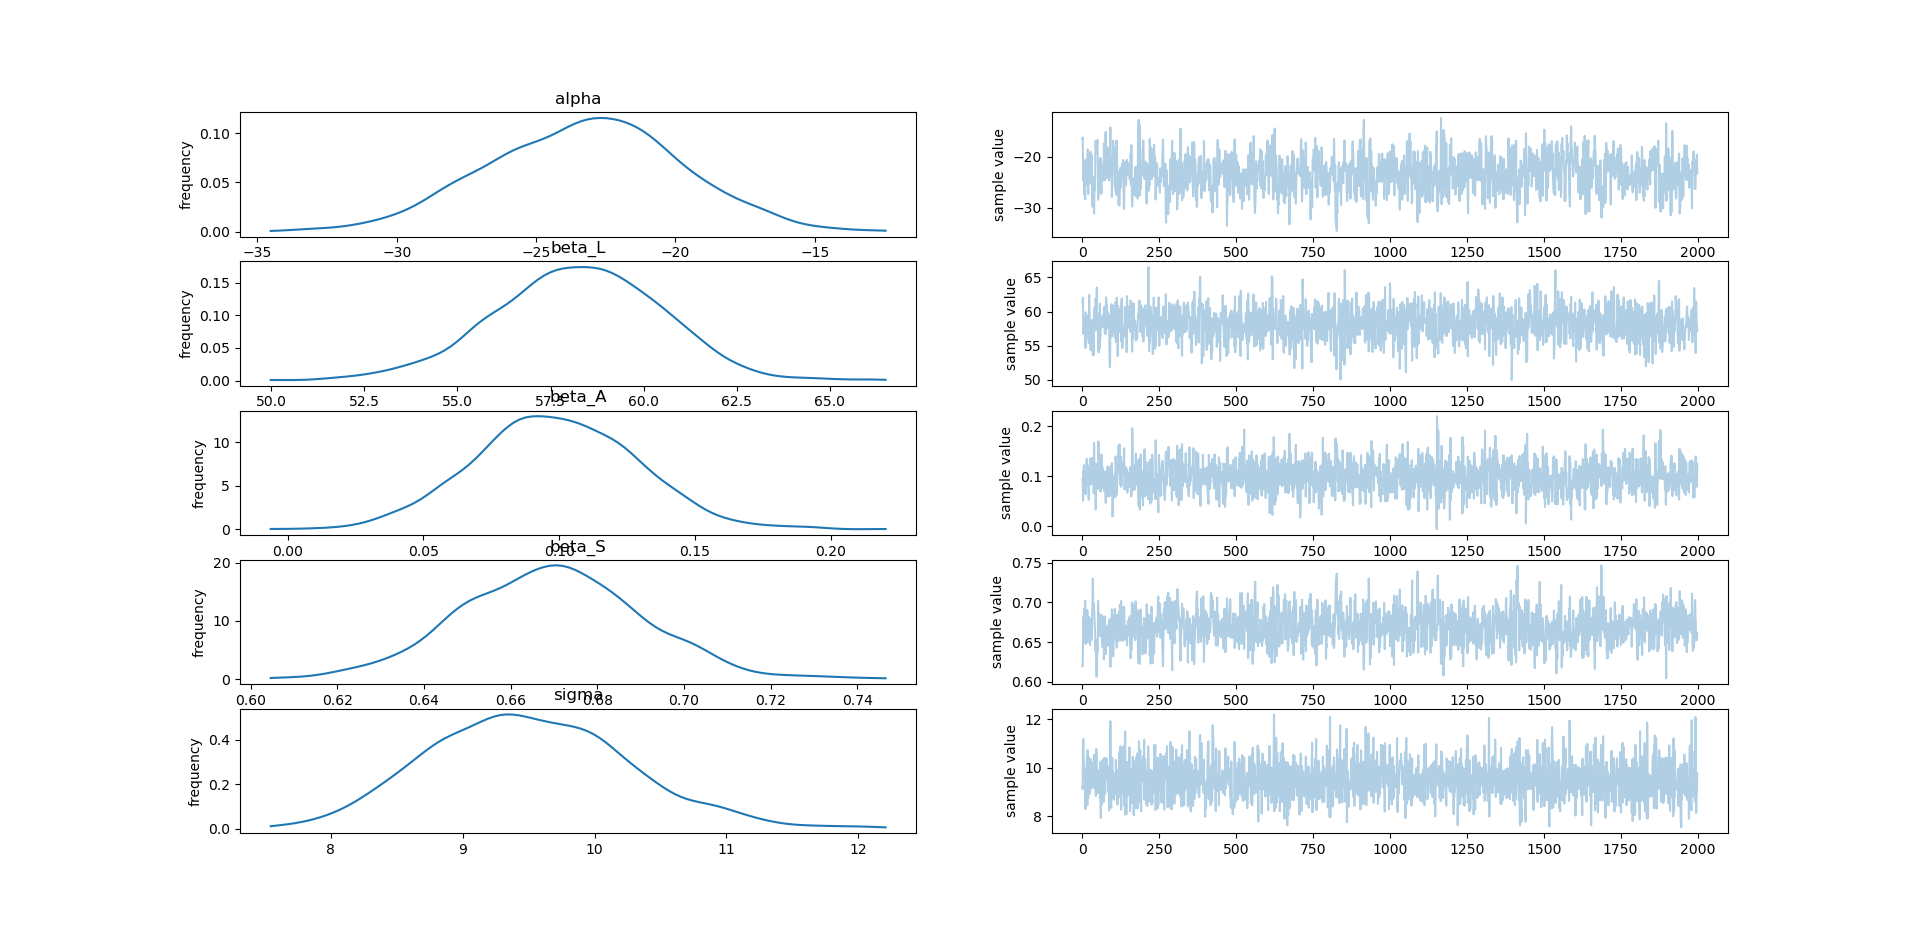
\includegraphics[width=\textwidth]{../q21/separated_features.png}
      \caption{Question 2.1 plot summary}
    \label{fig:2.1}
  \end{figure}


  \subsection{A less simple model (figs. \ref{fig:2.2} and \ref{tab:2.2})}
  Denoting that size has a positive effect on price does not affect performance. This is potentially due to the fact that the data already embodies this fact and explicitly stating it does not give us any new knowledge.

  \begin{figure}[htb]
    \centering
      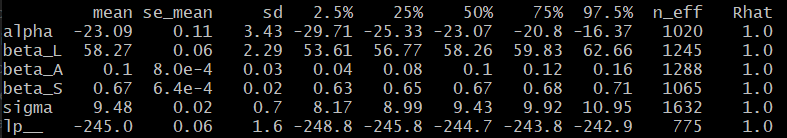
\includegraphics[width=\textwidth]{../q22/q22_table_summary.png}
      \caption{Question 2.2 posterior table summary}
    \label{tab:2.2}
  \end{figure}

  \begin{figure}[htb]
    \centering
      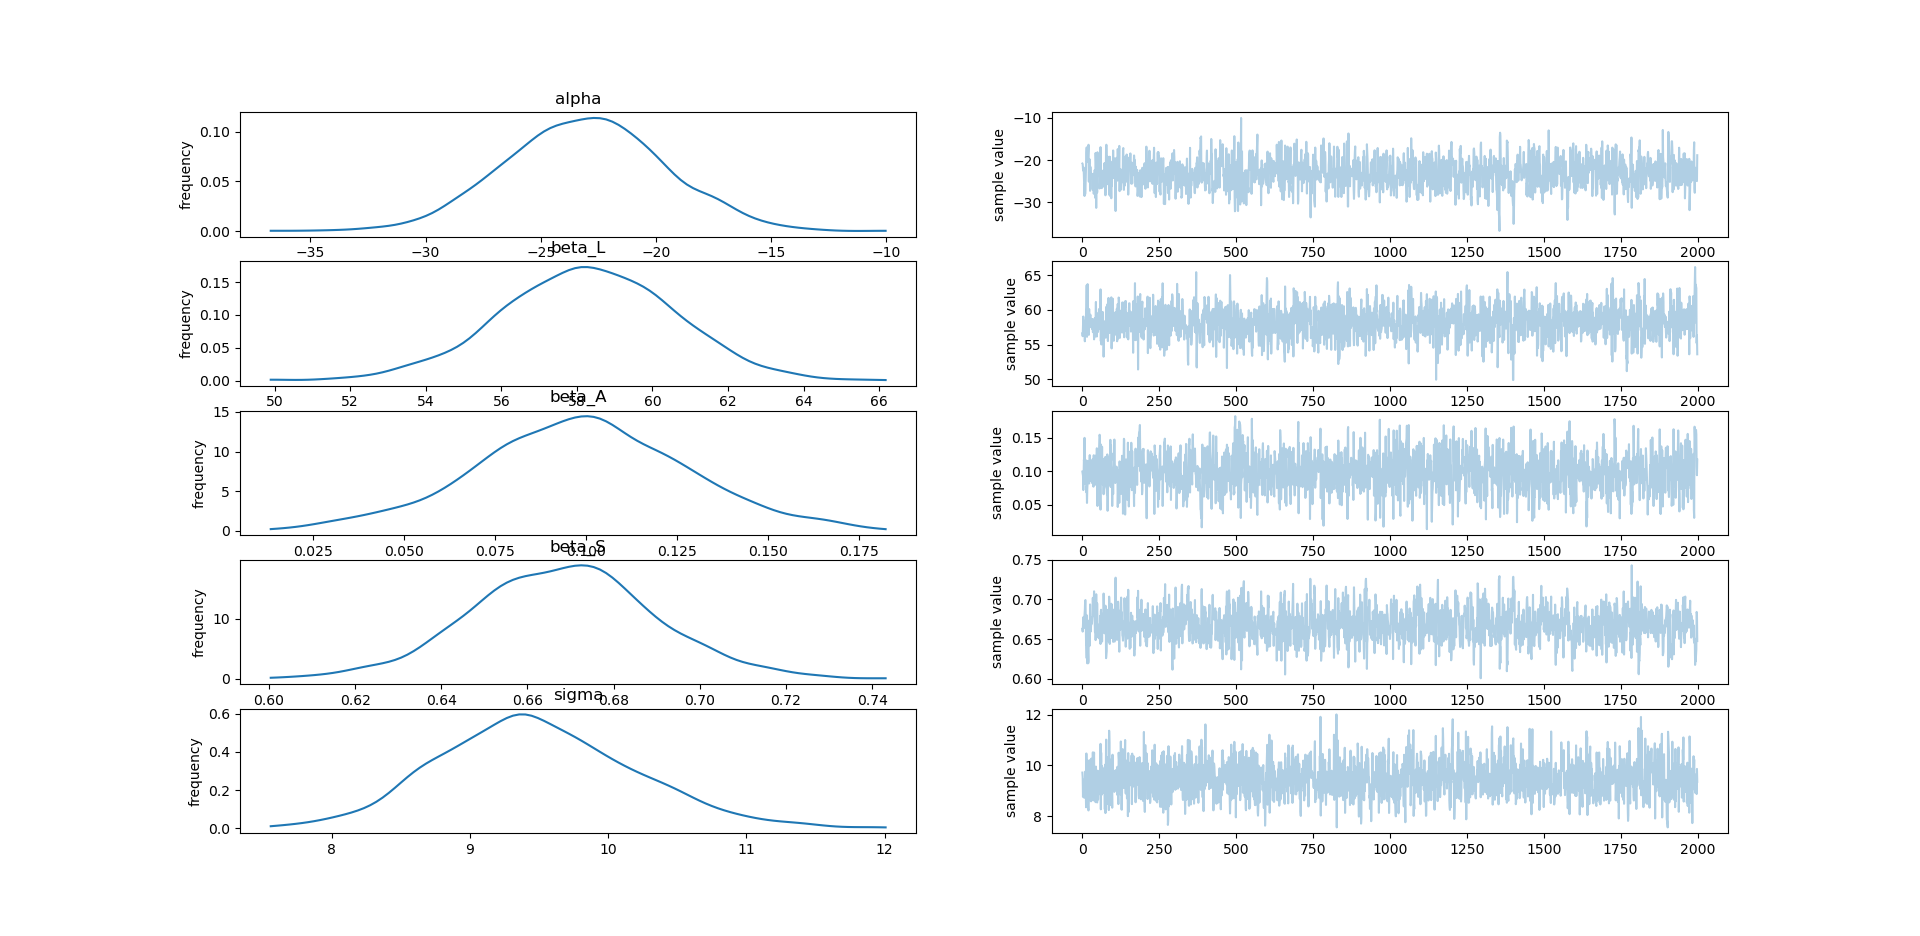
\includegraphics[width=\textwidth]{../q22/q22_plot_summary.png}
      \caption{Question 2.2 plot summary}
    \label{fig:2.2}
  \end{figure}

  \subsection{Two models (figs. \ref{fig:2.3_0},\ref{fig:2.3_1})}
  %TODO: Discuss the intercept values being so different
  Houses in 0 get cheaper with age, which was obfuscated in 2.2. Splitting also reduces noise. The higher certainty in our split models is also reflected by the superior \texttt{lp\_\_}.

  \begin{figure}[htb]
    \centering
    \begin{subfigure}[b]{\textwidth}
      \centering
      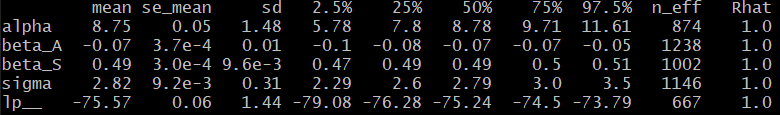
\includegraphics[width=\textwidth]{../q23/q23_table_summary_L0.png}
      \caption{posterior table summary}
    \end{subfigure}
    \hfill
    \begin{subfigure}[b]{\textwidth}
      \centering
      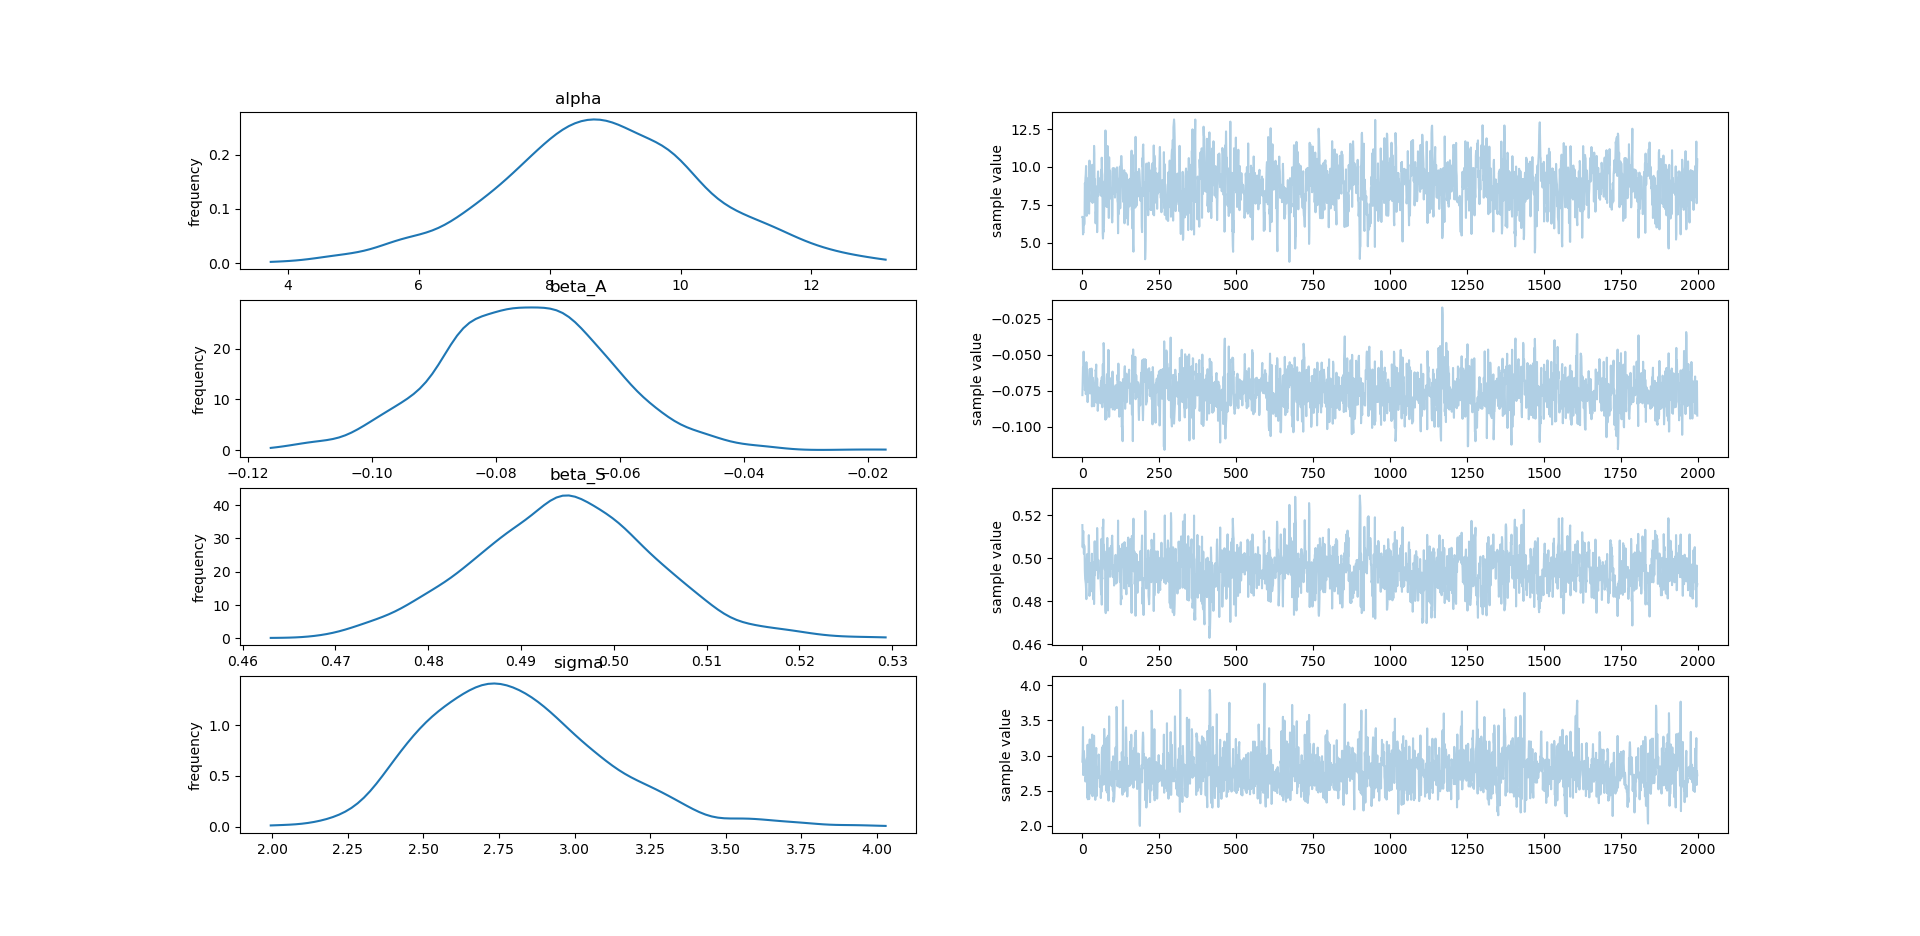
\includegraphics[width=\textwidth]{../q23/q23_plot_summary_L0.png}
      \caption{plot summary}
    \end{subfigure}
    \caption{Question 2.3 Locale 0}
    \label{fig:2.3_0}
  \end{figure}

  \begin{figure}[htb]
    \centering
    \begin{subfigure}[b]{\textwidth}
      \centering
      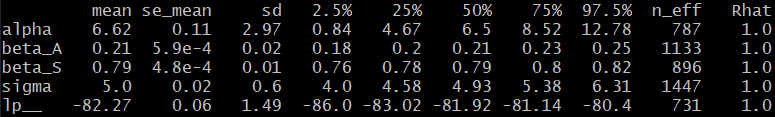
\includegraphics[width=\textwidth]{../q23/q23_table_summary_L1.png}
      \caption{posterior table summary}
    \end{subfigure}
    \hfill
    \begin{subfigure}[b]{\textwidth}
      \centering
      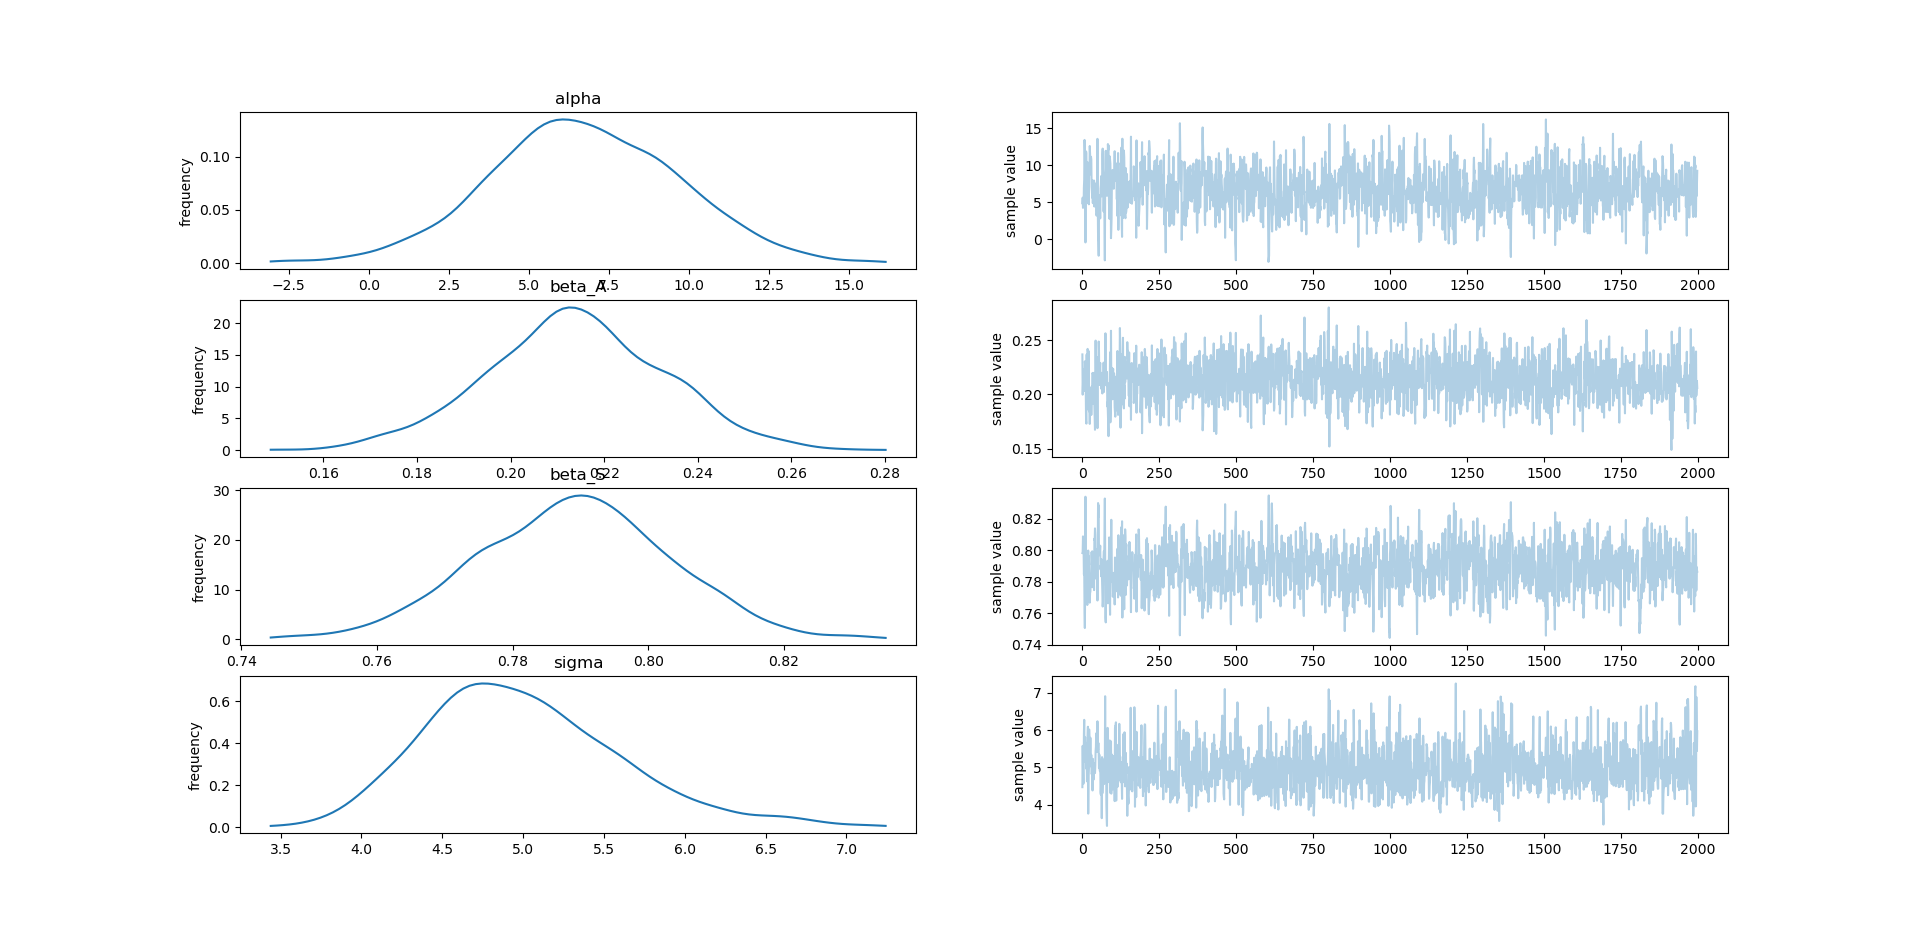
\includegraphics[width=\textwidth]{../q23/q23_plot_summary_L1.png}
      \caption{plot summary}
    \end{subfigure}
    \caption{Question 2.3 Locale 1}
    \label{fig:2.3_1}
  \end{figure}

  \subsection{A compromise model (figs. \ref{tab:2.4}, \ref{fig:2.4} \ref{fig:2.4_bnet})}
 
 % An intuitive formulation of this problem would be a model that permits each locale its own parameters, yet communicates general knowledge about the domain across the locales.
  We create a hierarchical model \parencite{MultilevelHM} that has variant slopes, but maintains the intercept across locales \(y_i = \alpha + \beta_{j[i]} x_i + \epsilon_i \) with all \(\epsilon \sim N(0,\sigma^{2})\) \parencite{VaryingAlpha}. With it we are able to capture the Age difference and still share knowledge  

  \begin{figure}[htb]
    \centering
      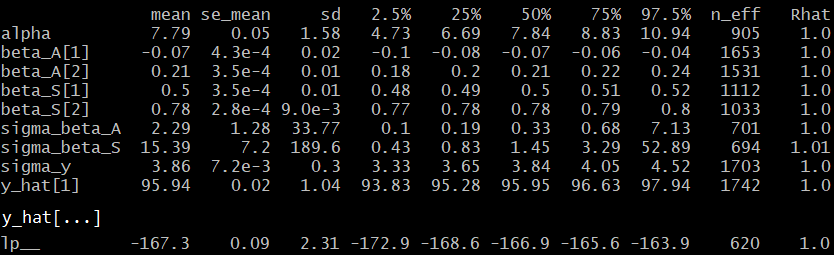
\includegraphics[width=0.95\textwidth]{../q24/q24_table_summary.png}
      \caption{Question 2.4 posterior table summary}
    \label{tab:2.4}
  \end{figure}

  \begin{figure}[htb]
    \centering
      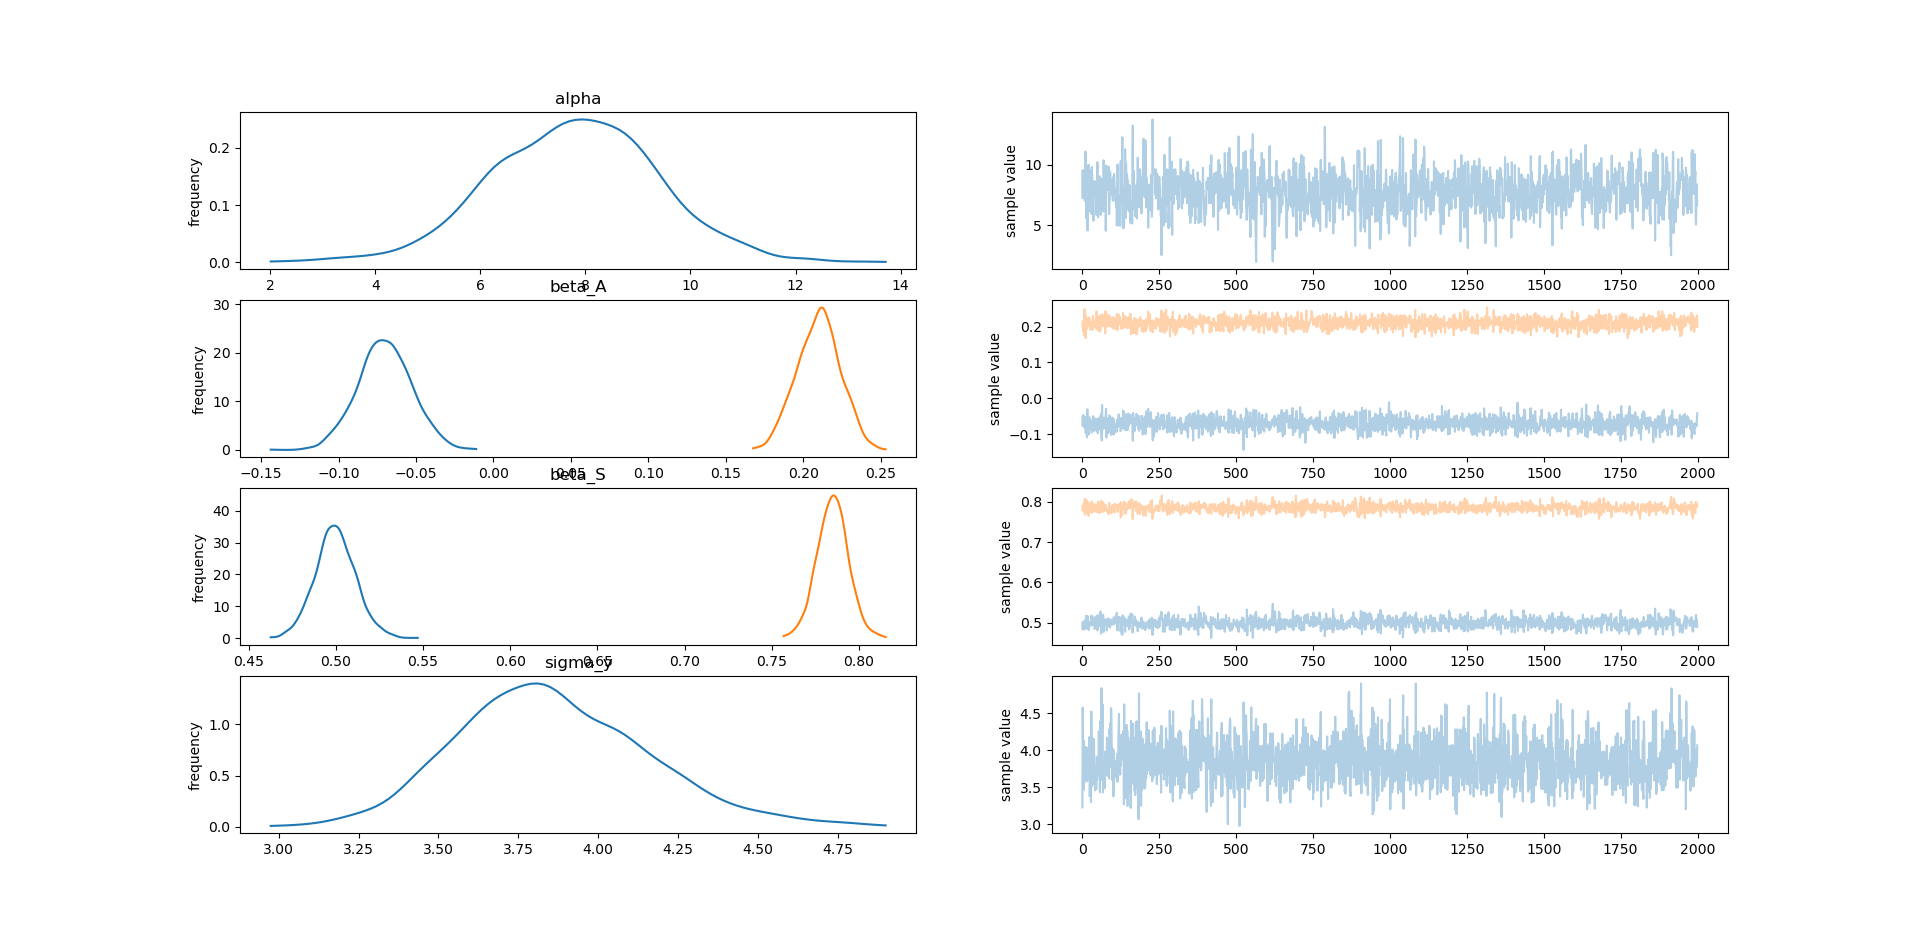
\includegraphics[width=\textwidth]{../q24/q24_plot_summary.png}
      \caption{Question 2.4 plot summary}
    \label{fig:2.4}
  \end{figure}

  \begin{figure}[htb]
    \centering
      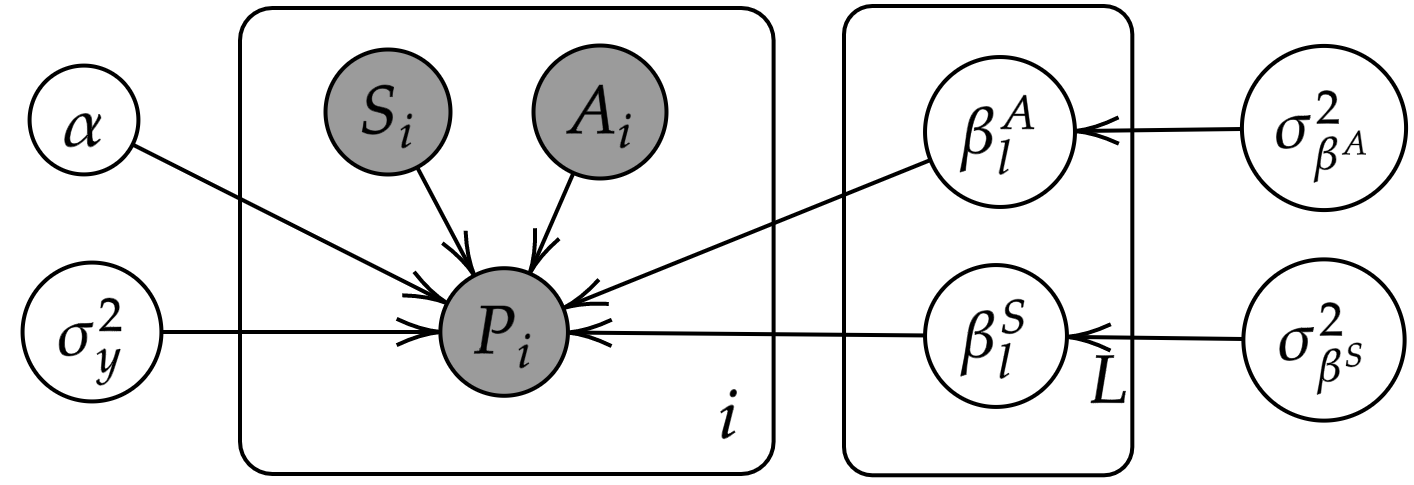
\includegraphics[width=\textwidth]{../q24/q24_bnet.png}
      \caption{Question 2.4 model as bayesian network}
    \label{fig:2.4_bnet}
  \end{figure}


\section{VB vs MCMC}

\textit{In fewer than 200 words overall: (i) describe Hamiltonian MCMC, (ii) describe variational inference as done in Stan and (iii) discuss the pros and cons of both approaches. (Any equations or figures do not count towards the word count.}
%TODO: how STAN uses HMCMC
%TODO: how VS is done
HMCMC approximates posteriors. VS approximates posteriors as a product of Gaussians \textbf{[[citation needed]]}.
VS is faster and has been optimised for large datasets \textbf{[[citation needed]]}, but if the true underlying distribution is not well approximated by a product of gaussians, VS will fail. MCMC is asymptotically precise yet is computationally intensive and multimodal distributions can confuse it. \textbf{[[citation needed]]}.


\section{Hidden Markov models}
\end{document}
\printbibliography